\section{Introduction}

Motivation:
\begin{itemize}
    \item In an aging society, exercising is an important factor to ensure a long and healthy life.
    \item This project will address the problem of learning user-specific heart rate response models for the use in (novel) smart training devices.
    \item Heart rates play an important role in improving the efficiency of physical training, but the data is highly individual-specific. The ability to reliably predicting heart rates from exercise workload can therefore allow for personalized training sessions. Model based planning, control and advanced monitoring techniques can also be built on top of such heart rate models. Finally, machine learning techniques allow learning non-linear models based on the recorded workload and environmental data, as well as adaptation to the environments through introducing additional variables such as track elevation and inclination.
\end{itemize}


\subsection{Recurrent Neural Networks (RNN)}
    \begin{figure}[H]
        \centering
        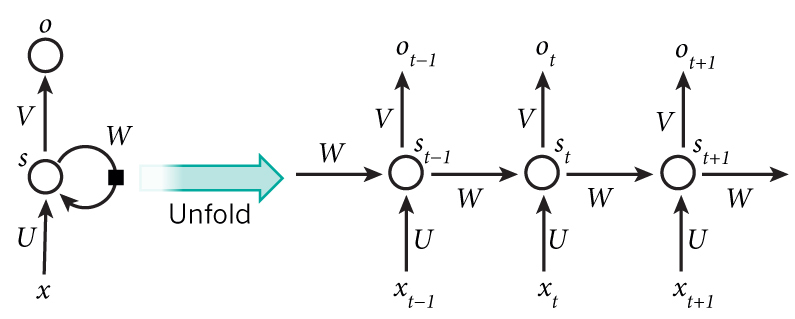
\includegraphics[width=0.8\linewidth]{../images/LeCun2015-deep_learning-fig5_rnn.jpg}
        \caption{A RNN and its forward computation unfolded in time \cite{LeCun2015}} \label{fig:rnn}
    \end{figure}
    \begin{itemize}
        \item RNN is a Deep Neural Network (DNN) which uses feedback connections to maintain historical information about previous elements of the input sequence \cite{Hochreiter:1997:LSM:1246443.1246450, LeCun2015}.
        \item Figure \ref{fig:rnn} illustrates a basic RNN. Node $s$ consists of neurons which receive inputs from other neurons at previous time steps. Element $o_t$ of the output sequence is mapped from element $x_t$ of the input sequence and information from previous time steps. Parameters $U$, $V$ and $W$ remain the same for every time step \cite{LeCun2015}.
        \item RNNs can be trained using ``Back-Propagation Through Time'' (BPTT). However, because the back-propagated gradients grow or shrink at each time step, the error signals of RNNs often either explode or vanish \cite{Hochreiter01gradientflow, LeCun2015}.
        \item The exploding gradient problem is often avoided by using gradient clipping, a technique which enforces a constraint over the norm of the gradient \cite{conf/icml/JozefowiczZS15}.
        \item Long Short-Term Memory (LSTM) and Gated Recurrent Unit (GRU) are popular RNN architectures which use memory cells to deal with the vanishing gradient problem.
    \end{itemize}

    \subsubsection*{Long Short-Term Memory}
    \begin{figure}[H]
        \centering
        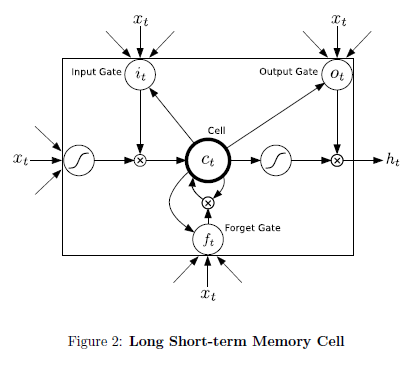
\includegraphics[width=0.7\linewidth]{../images/Graves13-fig2-lstm_arch.png}
        \caption{Long Short-Term memory cell \cite{DBLP:journals/corr/Graves13}} \label{fig:lstm}
    \end{figure}
    \begin{itemize}
        \item A naive approach to dealing with the vanishing error term is Constant Error Carousal (CEC), which uses an identity activation function and weights of 1.0 to enforce a local constant error flow for each hidden unit. However, this results in conflicts when learning input and output weights \cite{Hochreiter:1997:LSM:1246443.1246450}:
        \begin{itemize}
            \item Input weights need to store some inputs while ignoring irrelevant ones.
            \item Output weights need to release information in the hidden units at certain times while not disturbing the output neurons at others.
        \end{itemize}
        \item LSTM was first introduced as an extension of CEC, which includes multiplicative input and output gates to deal with the aforementioned conflicts \cite{Hochreiter:1997:LSM:1246443.1246450}.
        \item LSTM can sometimes fail to learn correctly sequences which are not segmented a priori into subsequences with clear beginning and ends, causing saturation of the output gate activation function. A forget gate was proposed by Felix Gers to allow the network for learning to reset itself when appropriate to deal with this saturation \cite{Gers:2000:LFC:1121912.1121915}.
        \item Figure \ref{fig:lstm} illustrates a LSTM memory cell. The Keras library used in the experiments for this report uses the LSTM formulation by Alex Graves \cite{Graves2012-385, DBLP:journals/corr/Graves13}:
        \begin{align*}
            i_t & = \sigma(W_{xi}x_t + W_{hi}h_{t-1} + W_{ci}c_{t-1} + b_i) \\
            f_t & = \sigma(W_{xf}x_t + W_{hf}h_{t-1} + W_{cf}c_{t-1} + b_f) \\
            c_t & =  f_t c_{t-1} + i_t\tanh(W_{xc}x_t + W_{hc}h_{t-1} + b_c) \\
            o_t & = \sigma(W_{xo}x_t + W_{ho}h_{t-1} + W_{co}c_{t} + b_o) \\
            h_t & = o_t \tanh(c_t)
        \end{align*}
        where $\sigma$ is the sigmoid function; $i, f, o, c$ are in turn input gate, forget gate, output gate, and cell input activation vectors, which are of the same size as the hidden vector $h$. The weight matrices have subscripts representing the elements they connect (i.e. $W_{xo}$ is for input-output gate connection).
    \end{itemize}

    \subsubsection*{Gated Recurrent Unit}


\subsection{Prior Work}
